% Source: tex/chapters/ch06/05_ソフトウェアエンジニアリング運用計画.tex
\subsubsection{開発環境と運用環境}

ソフトウェアプロセスでは、開発環境、試験環境または品質保証環境、事前本番環境、本番環境が使われる。品質を作り込み、本番リリースのリスクを下げるには、これらの環境が一貫しており、本番環境と同期している必要がある。

\par\smallskip\noindent\refstepcounter{table}\label{tab:ch06-05}\textbf{表 \thetable: 第06章 ソフトウェアエンジニアリング運用 表05}\par\smallskip
\begin{longtable}{L{35mm}L{115mm}}
\toprule
環境 & 目的 \\
\midrule
開発環境 & 開発者がコードを書き、単体試験や小規模な確認を行う環境である。 \\
試験・品質保証環境 & 統合試験、品質保証、回帰試験、自動試験を実行する環境である。 \\
事前本番環境 & 本番に近い条件で、配備手順、性能、運用手順を確認する環境である。 \\
本番環境 & 実際の利用者にサービスを提供する環境である。 \\
\bottomrule
\end{longtable}

DevOpsでは、これらの環境を単一のコードリポジトリから自動的に作成することが推奨される。すべての環境が同じコード源から作られれば、環境差分による不具合を減らせる。これがインフラストラクチャのコード化につながる。

\begin{figure}[htbp]
\centering
\IfFileExists{assets/fig-ch06-04.png}{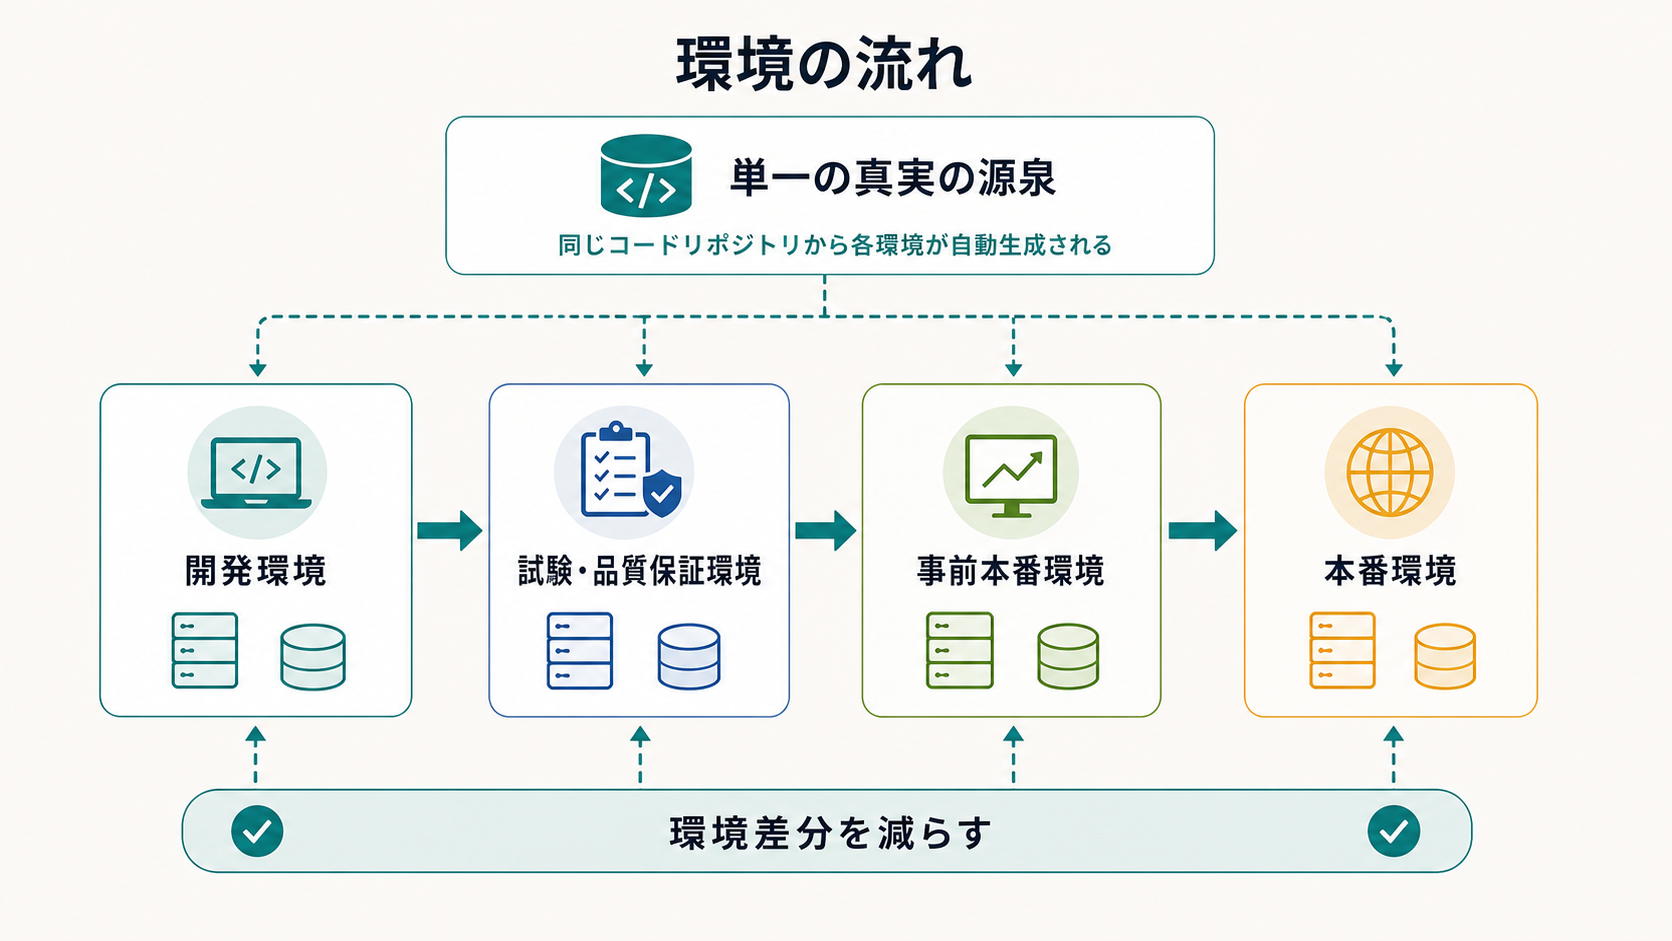
\includegraphics[width=0.96\linewidth]{assets/fig-ch06-04.png}}{\fbox{\parbox[c][48mm][c]{0.9\linewidth}{\centering 画像生成待ち\\環境の流れ}}}
\caption{環境の流れ}
\label{fig:ch06-04}
\end{figure}
